\section{Математическая модель манипулятора}\label{part_math_model_of_robot}

\subsection{Кинематика манипулятора}\label{part_kinematics}

% TODO Тут обосновать зачем нужна кинематика манипулятора

Представим рассматриваемый манипулятор в виде последовательной кинематической цепи, каждое звено которой входит в состав одной или двух кинематических пар (КП). Все КП вращательные, V-класса -- цилиндрические шарниры. Принципиальная схема изображена на рисунке~\ref{img:kinematics} a.

\begin{figure}[h!]
	\begin{minipage}[h]{0.5\linewidth}
		\center{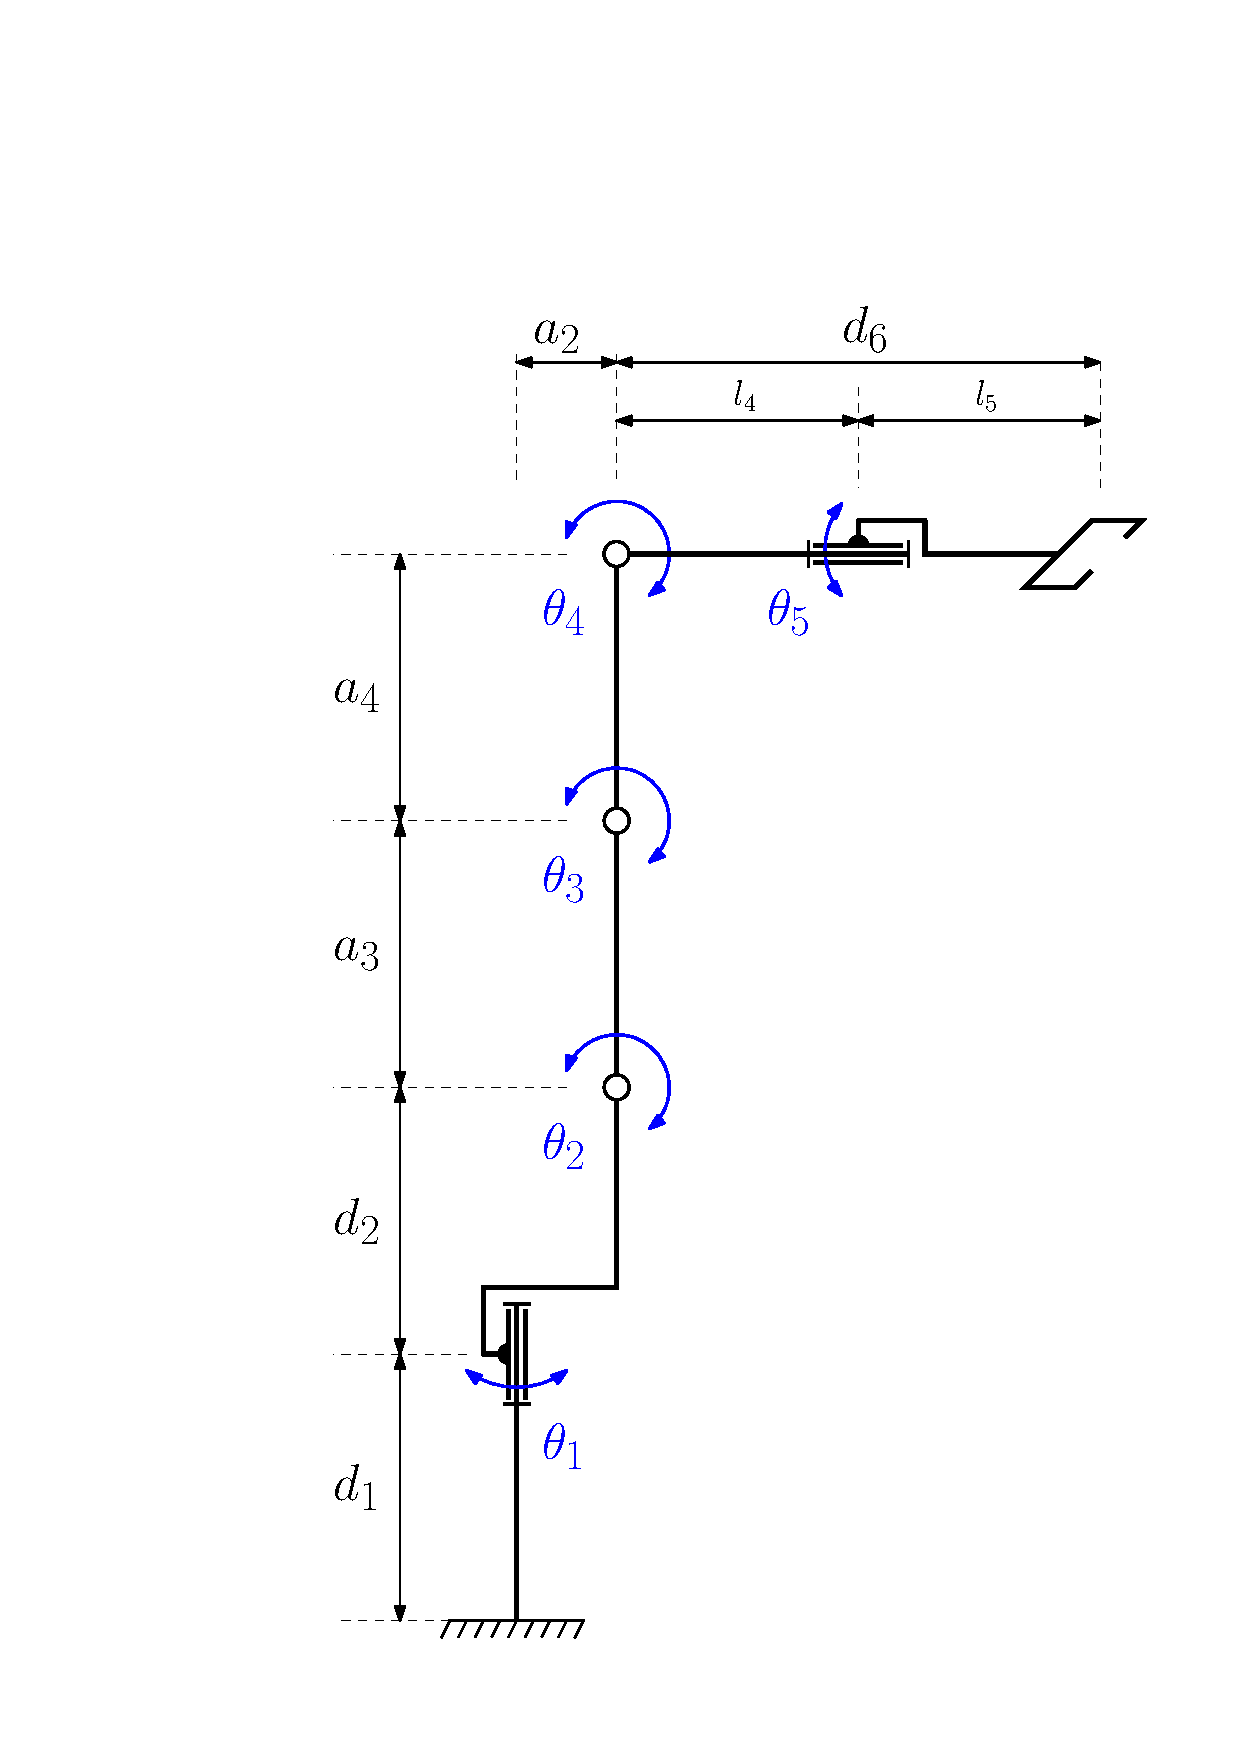
\includegraphics[width=0.95\linewidth]{kinematics_schema.pdf} \\ а) кинематическая схема}
	\end{minipage}
	\hfill
	\begin{minipage}[h]{0.5\linewidth}
		\center{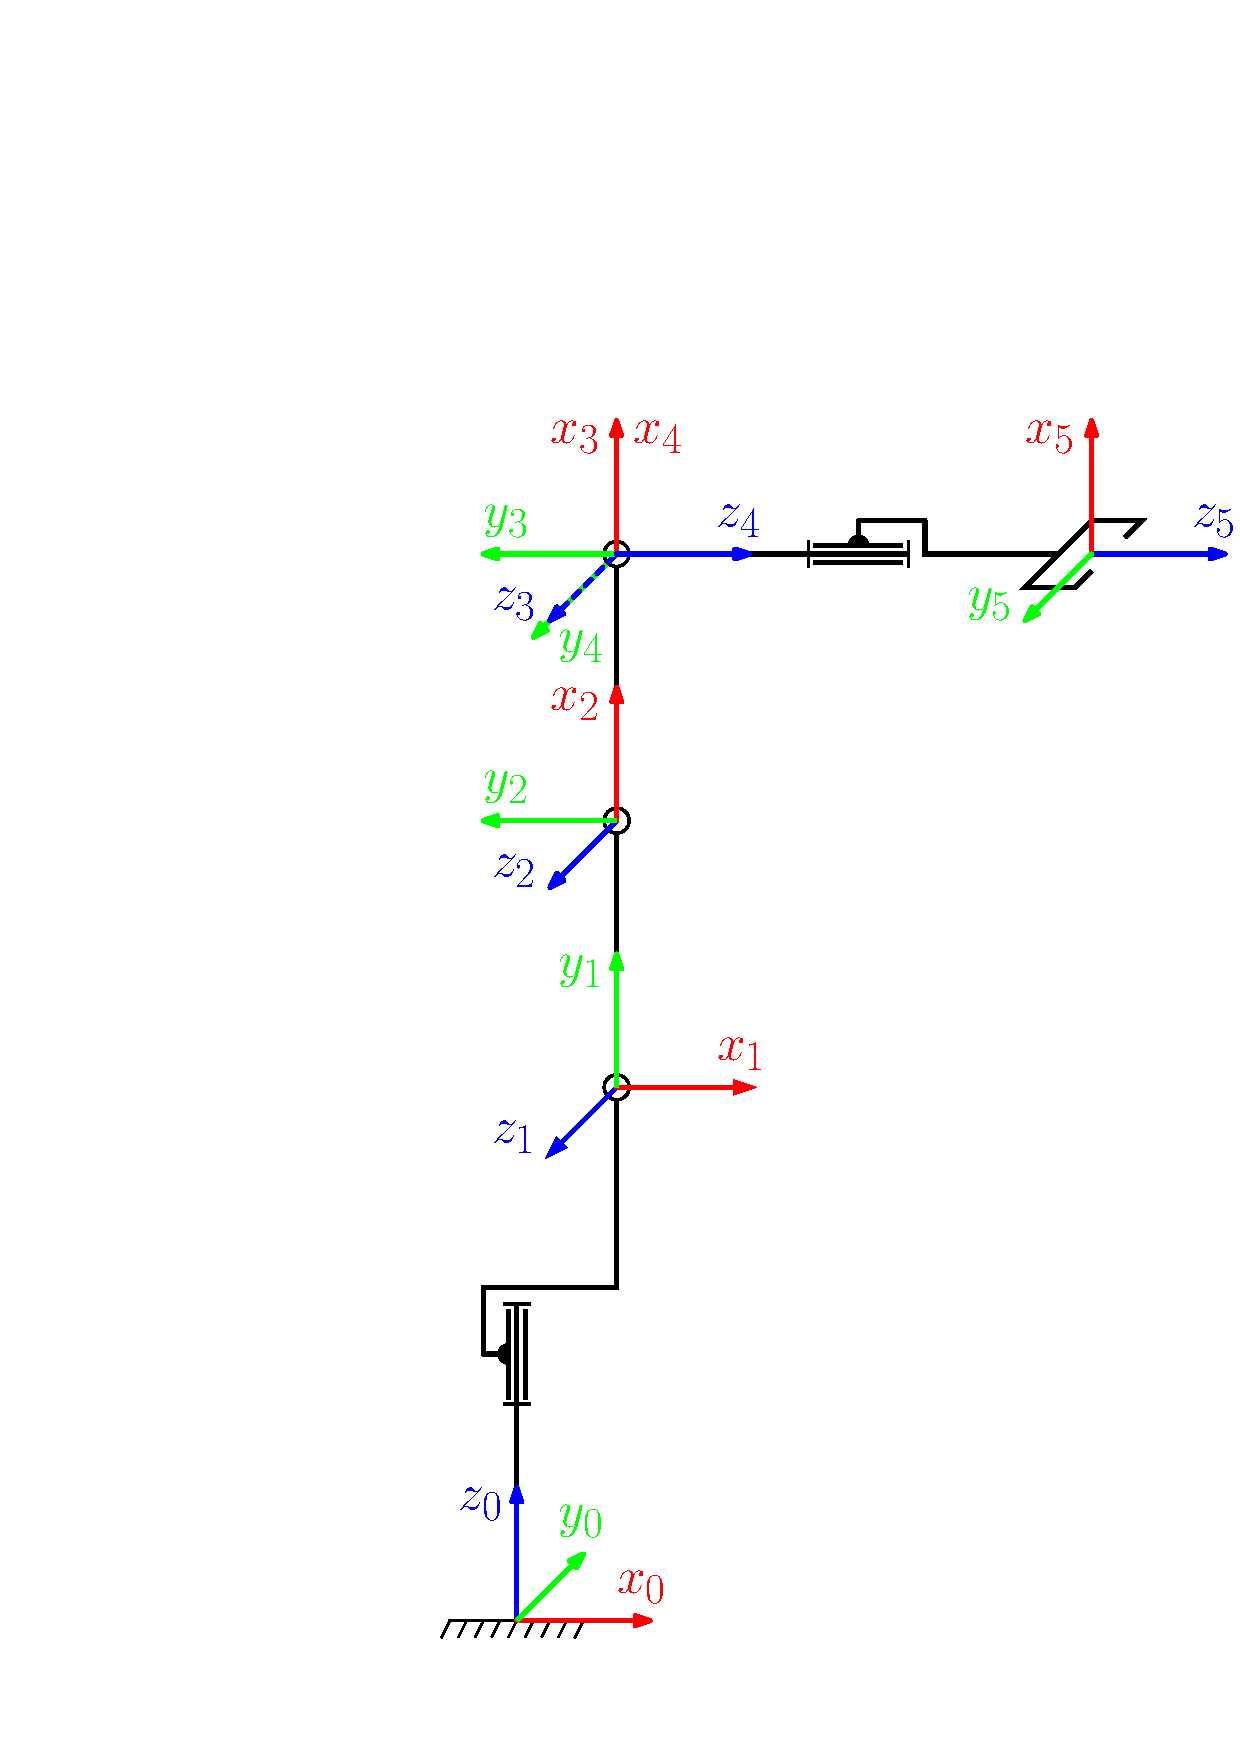
\includegraphics[width=0.95\linewidth]{kinematics_frames.pdf} \\ б) схема расположения СК КП}
	\end{minipage}
	\caption{Схемы}
	\label{img:kinematics}
\end{figure}

Звенья будем рассматривать как абсолютно твердые тела, определяющие связь между двумя соседними шарнирами. Для описания шарнирных соединений между смежными звеньями воспользуемся методом Денавита и Хартенберга (ДХ-представление), который может быть представлен, как последовательность из двух описанных ниже шагов\footnote{Представление Денавита-Хартенберга состоит в формировании однородной матрицы преобразования, имеющей размерность~$4 \times 4$ и описывающей положение системы координат каждого звена относительно системы координат предыдущего звена.}.


Первым шагом, следует сформировать системы координат для каждой~КП, руководствуясь следующими правилами:

\begin{enumerate}
	\item ось $z_{i-1}$ направлена вдоль оси $i$-ой КП;
	\item ось $x_i$ параллельна общему перпендикуляру: $x_i = z_i \times z_{i-1}$. Если оси $z_i$ и $z_{i-1}$ пересекаются, то $x_i$ выбирается, как нормаль к образованной ими плоскости;
	
	\item ось $y_i$ дополняет оси $z_i$ и $x_i$ до правой декартовой системы координат. 
\end{enumerate}

Вторым шагом, нужно определить параметры ДХ:

\begin{enumerate}
	\item $a_i$ -- расстояние от $z_{i-1}$ до $z_i$ вдоль $x_i$;
	\item $\alpha_i$ -- угол от $z_{i-1}$ до $z_i$ вокруг $x_i$;
	\item $d_i$ -- расстояние от $x_{i-1}$ до $x_i$ вдоль $z_{i-1}$;
	\item $\theta_i$ -- угол от $x_{i-1}$ до $x_i$ вокруг $z_{i-1}$.
\end{enumerate}

Таким образом, ДХ-представление твердых звеньев зависит от четырех геометрических параметров, соответствующих каждому звену. Эти четыре параметра полностью описывают любое вращательное или поступательное движение. 

Для вращательных КП параметры $d_i$, $a_i$ и $\alpha_i$ не изменяются и являются их геометрическими размерами. В то время,  как $\theta_i$ переменная величина, изменяющаяся при вращении $i$-го звена относительно $(i-1)$-го.

Для каждого звена этот алгоритм формирует ортонормированную систему координат. Системы координат нумеруются в порядке возрастания от основания к схвату манипулятора. Для обследуемого манипулятора, выбранные системы координат изображены на рисунке~\ref{img:kinematics} б. 

Параметры ДХ указаны в таблице~\ref{table_DH_params}

\begin{table}[h!]
	\caption{Параметры Денавита-Хартенберга}
	\begin{center}
		\begin{tabular}{|c|c|c|c|c|}
			\hline
			Звено 	& $a_i$ & $\alpha_i$ & $d_i$ & $\theta_i$\\
			\hline
			1 		& $0$ & $0$ 	& $d_1$ & $0$\\
			\hline
			2  		& $a_2$ & $\pi/2$ & $d_2$ & $\theta_1$\\
			\hline	
			3 		& $a_3$ & $0$ 	& $0$ 	& $\theta_2+\pi/2$\\
			\hline
			4 		& $a_4$ & $0$ 	& $0$ 	& $\theta_3$\\
			\hline
			5 		& $0$ & $\pi/2$ & $0$ 	& $\theta_4$\\
			\hline
			6 		& $0$ & $0$ 	& $d_6$ & $\theta_5$\\
			\hline
		\end{tabular}
	\end{center}
	\label{table_DH_params}
\end{table}

Взаимное расположение соседних звеньев описывается однородной матрицей преобразования~\eqref{DH_matrix_A} размерностью $4 \times 4$, которая формируется в соответствии с формулой~\eqref{DH_matrix}.

\begin{equation}\label{DH_matrix}
^{i}A_{i+1} = R_{z_i, \theta_i} \cdot T_{z_i, d_i} \cdot T_{x_i, a_i} \cdot R_{x_i, \alpha_i}	
\end{equation}
где $R_{z_i, \theta_i}$~--- матрица поворота вокруг оси $z_i$ на угол $\theta_i$, $T_{z_i, d_i}$~--- матрица трансформации вдоль оси $z_i$ на расстояние $d_i$, $T_{x_i, a_i}$~---матрица трансформации вдоль оси $x_i$ на расстояние $a_i$,  $R_{x_i, \alpha_i}$~--- матрица поворота вокруг оси $x_i$ на угол $\alpha_i$.

\begin{equation}\label{DH_matrix_A}
^{i}A_{i+1} =
\begin{bmatrix}
R_{3 \times 3} & p_{3 \times 1}\\
0_{1 \times 3} & 1
\end{bmatrix}
\end{equation}
где $R_{3 \times 3}$~--- матрица поворота СК$_i$ в СК$_{i+1}$, $p_{3 \times 1}$~--- вектор соединяющий СК$_i$ и СК$_{i+1}$.

Для описания движения манипулятора, в робототехнике решаются две основные задачи кинематики: прямая и обратная.
 
Решением прямой задачи, находят положение схвата манипулятора в декартовой системе координат, при заданных обобщенных координатах.

Решение обратной задачи позволяет найти обобщенные координаты при заданном положении и ориентации схвата.

\subsubsection{Прямая задача кинематики}\label{part_kinematics_forward}

\if 0
% удалить
Представим прямую задачу кинематики функцией $f$, которая определяет зависимость между  конфигурационным и рабочим пространствами манипулятора:
\begin{equation}
	x = f(q)
\end{equation}
где $x \in \mathbb{R}^6$ --- вектор положения и ориентации схвата в рабочем пространстве, $q \in \mathbb{R}^5$ --- вектор обобщенных координат в конфигурационном пространстве манипулятора.
\fi

Представим прямую задачу кинематики (ПЗК) манипулятора выражением:
\begin{equation}\label{fk}
	^0A_6 = \prod^{6}_{i=1}{^{i-1}A_i(q_i)} = ^0A_1 \cdot ^1A_2 \cdot ^2A_3 \cdot ^3A_4 \cdot ^4A_5 \cdot ^5A_6
\end{equation}
где $^0A_6$~--- матрица $4 \times 4$, первые $3$ столбца которой представляют ориентацию, последний --- положение схвата; $^{i-1}A_i$~--- однородная матрица преобразования из $(i-1)$ в $i$-ую СК в общем виде:
\begin{equation}
	^{i-1}A_i = 
	\left[\begin{matrix}
	\cos{\left (\theta_i \right )} & - \sin{\left (\theta_i \right )} \cos{\left (\alpha_i \right )} & \sin{\left (\alpha_i \right )} \sin{\left (\theta_i \right )} & a_{i} \cos{\left (\theta_i \right )}\\
	\sin{\left (\theta_i \right )} & \cos{\left (\alpha_i \right )} \cos{\left (\theta_i \right )} & - \sin{\left (\alpha_i \right )} \cos{\left (\theta_i \right )} & a_{i} \sin{\left (\theta_i \right )}\\
	0 & \sin{\left (\alpha_i \right )} & \cos{\left (\alpha_i \right )} & d_{i}\\
	0 & 0 & 0 & 1
	\end{matrix}\right]
\end{equation}

Теперь, учитывая ДХ-параметры из таблицы~\ref{DH_matrix} находим матрцы преобразования СК, рисунок~\ref{img:kinematics} б.

\begin{align*}
	^0A_1 &=& 
	\left[\begin{matrix}1 & 0 & 0 & 0\\0 & 1 & 0 & 0\\0 & 0 & 1 & d_{1}\\0 & 0 & 0 & 1\end{matrix}\right]; 
	^1A_2 =
 	\left[\begin{matrix}c_{\theta_1} & 0 & s_{\theta_1} & a_{2} c_{\theta_1}\\s_{\theta_1} & 0 & - c_{\theta_1} & a_{2} s_{\theta_1}\\0 & 1 & 0 & 0\\0 & 0 & 0 & 1\end{matrix}\right];
	^2A_3 =
	\left[\begin{matrix}c_{\theta_2} & - s_{\theta_2} & 0 & a_{3} c_{\theta_2}\\s_{\theta_2} & c_{\theta_2} & 0 & a_{3} s_{\theta_2}\\0 & 0 & 1 & d_{2}\\0 & 0 & 0 & 1\end{matrix}\right];
	\\
	^3A_4 &=& 
	\left[\begin{matrix}c_{\theta_3} & - s_{\theta_3} & 0 & a_{4} c_{\theta_3}\\s_{\theta_3} & c_{\theta_3} & 0 & a_{4} s_{\theta_3}\\0 & 0 & 1 & 0\\0 & 0 & 0 & 1\end{matrix}\right];
	^4A_5 =
	 \left[\begin{matrix}c_{\theta_4} & 0 & s_{\theta_4} & 0\\s_{\theta_4} & 0 & - c_{\theta_4} & 0\\0 & 1 & 0 & 0\\0 & 0 & 0 & 1\end{matrix}\right];
	^5A_6 =
	\left[\begin{matrix}c_{\theta_5} & - s_{\theta_5} & 0 & 0\\s_{\theta_5} & c_{\theta_5} & 0 & 0\\0 & 0 & 1 & d_{6}\\0 & 0 & 0 & 1\end{matrix}\right]
\end{align*}

Таким образом, для любого вектора $q$, позьзуясь выражением~\eqref{fk} и ДХ-параметрами маниплятора, можно определить однозначное положение и ориентацию схвата манипулятора в пространстве.

Для проверки, зададим вектор обобщенных координат:
\begin{equation}
	q =
	\begin{bmatrix}
	\theta_1 & \theta_2 & \theta_3 & \theta_4 & \theta_5
	\end{bmatrix}
	=
	\begin{bmatrix}
	0 & 0 & 0 & 90 & 0
	\end{bmatrix}
\end{equation}

\begin{figure}[h]
	\centering
	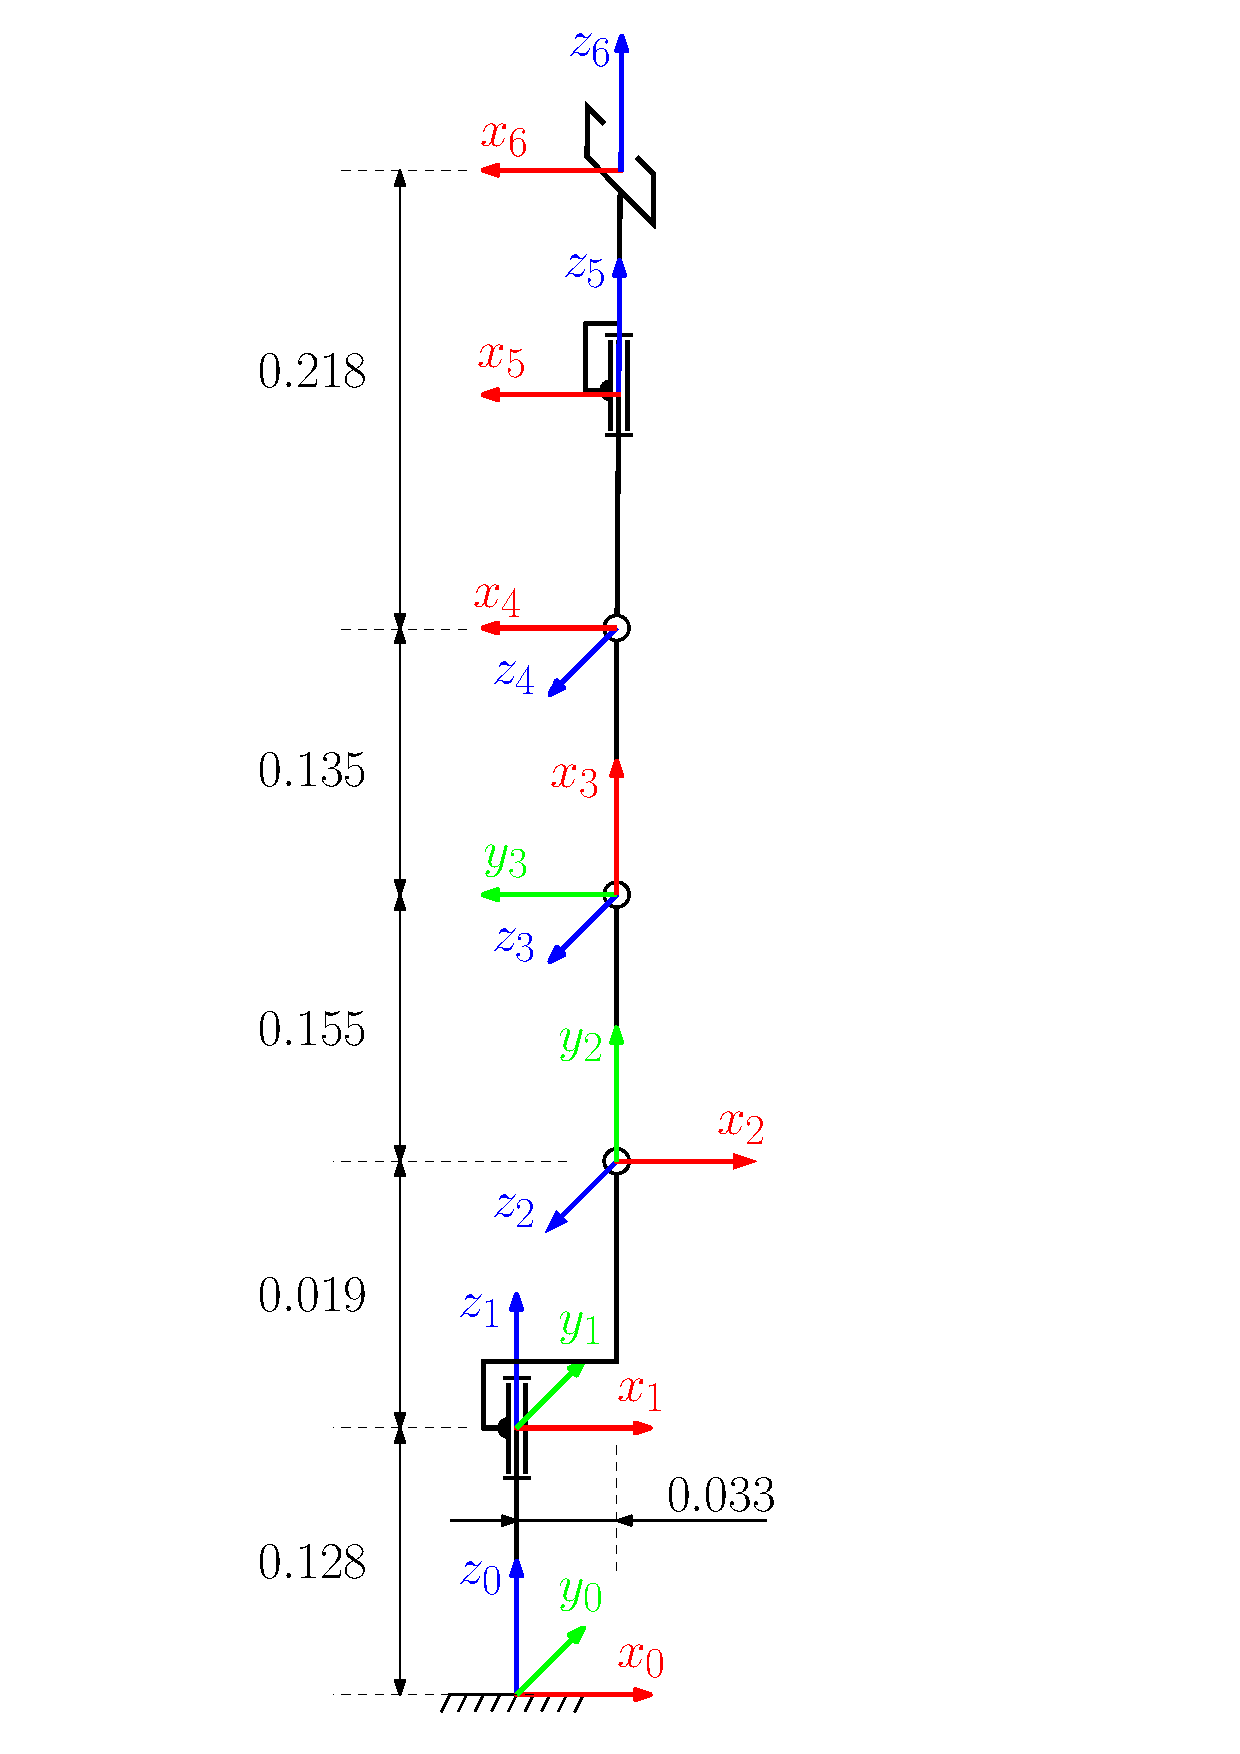
\includegraphics[width=0.2\textwidth]{kinematics_check.pdf}
	\caption{Конфигурация манипулятора для заданного вектора $q$}
	\label{kinematics_check}
\end{figure}

В результате решения ПЗК должны получить:
\begin{align*}
	p = 
	\begin{bmatrix}
		0.033\\
		0\\
		0.655 
	\end{bmatrix},
	o =
	\begin{bmatrix}
		0\\
		0\\
		180
	\end{bmatrix}, 
\end{align*}
где $p$~--- положение схвата, $o$~--- ориентация схвата (крен, рыскание, тангаж).

Вычислим матрицу $^0A_6$:
\begin{equation}
	^0A_6 = 
	\left[\begin{matrix}-1 & 0 & 0 & 0.033\\0 & -1 & 0 & 0\\0 & 0 & 1 & 0.655\\0 & 0 & 0 & 1\end{matrix}\right]
\end{equation}

Из приведенного примера следует, что ДХ-параметры и матрицы трансформации найдены верно.

\subsubsection{Обратная задача кинематики}\label{part_kinematics_inverse}

% удалтить
Обратную задачу кинематики представим, как функцию $g = f^{-1}$, представляющую переход из рабочего в конфигурационное пространство:
\begin{equation}
\textbf{q} = g(\textbf{p}, \textbf{o}) = f^{-1}(\textbf{p}, \textbf{o})
\end{equation}
где вектор $\textbf{p}$~--- заданное положение в рабочем пространстве, вектор $\textbf{o}$~--- заданная ориентация системы координат схвата.

Для удобства будем пользоваться однородными матрицами преобразования.
Матрица, задающая положение и ориентацию схвата в системе координат базы, имеет вид:
\begin{equation}\label{ik}
	^0T_6 =
	\left[\begin{matrix}
	r_{11} & r_{12} & r_{13} & p^{x}\\
	r_{21} & r_{22} & r_{23} & p^{y}\\
	r_{31} & r_{32} & r_{33} & p^{z}\\
	0 & 0 & 0 & 1
	\end{matrix}\right]
\end{equation}

Приравняв матрицу $^0T_6$ и правую часть выражения~\eqref{fk} и домножив с обеих сторон на $(^0A_1 \cdot ^1A_2)^{-1}$, получим выражение:
\begin{equation}
	(^0A_1 \cdot ^1A_2)^{-1} \cdot ^0T_6 = ^2A_3 \cdot ^3A_4 \cdot ^4A_5 \cdot ^5A_6
\end{equation}
где левая часть:
\begin{align*}
	^2T_6 &= 
	\left[\begin{matrix}
		r_{11} c_{1} + r_{21} s_{1} & r_{12} c_{1} + r_{22} s_{1} & r_{13} c_{1} + r_{23} s_{1} & - a_{2} + p^{x} c_{1} + p^{y} s_{1}\\
		r_{31} & r_{32} & r_{33} & - d_{1} - d_{2} + p^{z}\\
		r_{11} s_{1} - r_{21} c_{1} & r_{12} s_{1} - r_{22} c_{1} & r_{13} s_{1} - r_{23} c_{1} & p^{x} s_{1} - p^{y} c_{1}\\
		0 & 0 & 0 & 1\end{matrix}\right],
\end{align*}
правая часть:
\begin{align*}
	^2A_6 &=
	\left[\begin{matrix}
		c_{5} c_{234} & - s_{5} c_{234} & s_{234} & a_{3} c_{2} + a_{4} c_{23} + d_{6} s_{234}\\
		s_{234} c_{5} & - s_{5} s_{234} & - c_{234} & a_{3} s_{2} + a_{4} s_{23} - d_{6} c_{234}\\
		s_{5} & c_{5} & 0 & 0\\
		0 & 0 & 0 & 1
	\end{matrix}\right].
\end{align*}

Теперь, приравнивая элементы с одинаковыми индексами получим уравнения, из которых найдем обобщенные координаты.

Из равенства элементов $(3,4)$: 
\begin{equation}
	p^{x} s_{1} - p^{y} c_{1} = 0
\end{equation}

Найдем $\theta_1$:
\begin{equation}
	\theta_1 = Atan2(p^y, p^x)
\end{equation}

Из равенств элементов $(3,1)$ и $(3,2)$:
\begin{align*}
	s_{5} = r_{11} s_{1} - r_{21} c_{1},\\
	c_{5} =  r_{12} s_{1} - r_{22} c_{1}
\end{align*}

Вычислим $\theta_5$:
\begin{equation}
	\theta_5 = Atan2(r_{11} s_{1} - r_{21} c_{1}, r_{12} s_{1} - r_{22} c_{1})
\end{equation}

Из равенств элементов $(2,3)$ и $(1,3)$:
\begin{align*}
	c_{234} &= -r_{33},\\
	s_{234} &= r_{13} c_{1} + r_{23} s_{1}
\end{align*}

Вычислим $\theta_{234}$:
\begin{equation}
	\theta_{234} = Atan2(r_{13} c_{1} + r_{23} s_{1}, -r_{33}) 
\end{equation}

Далее применим геометрический подход.

\begin{figure}[h!]
	\centering
	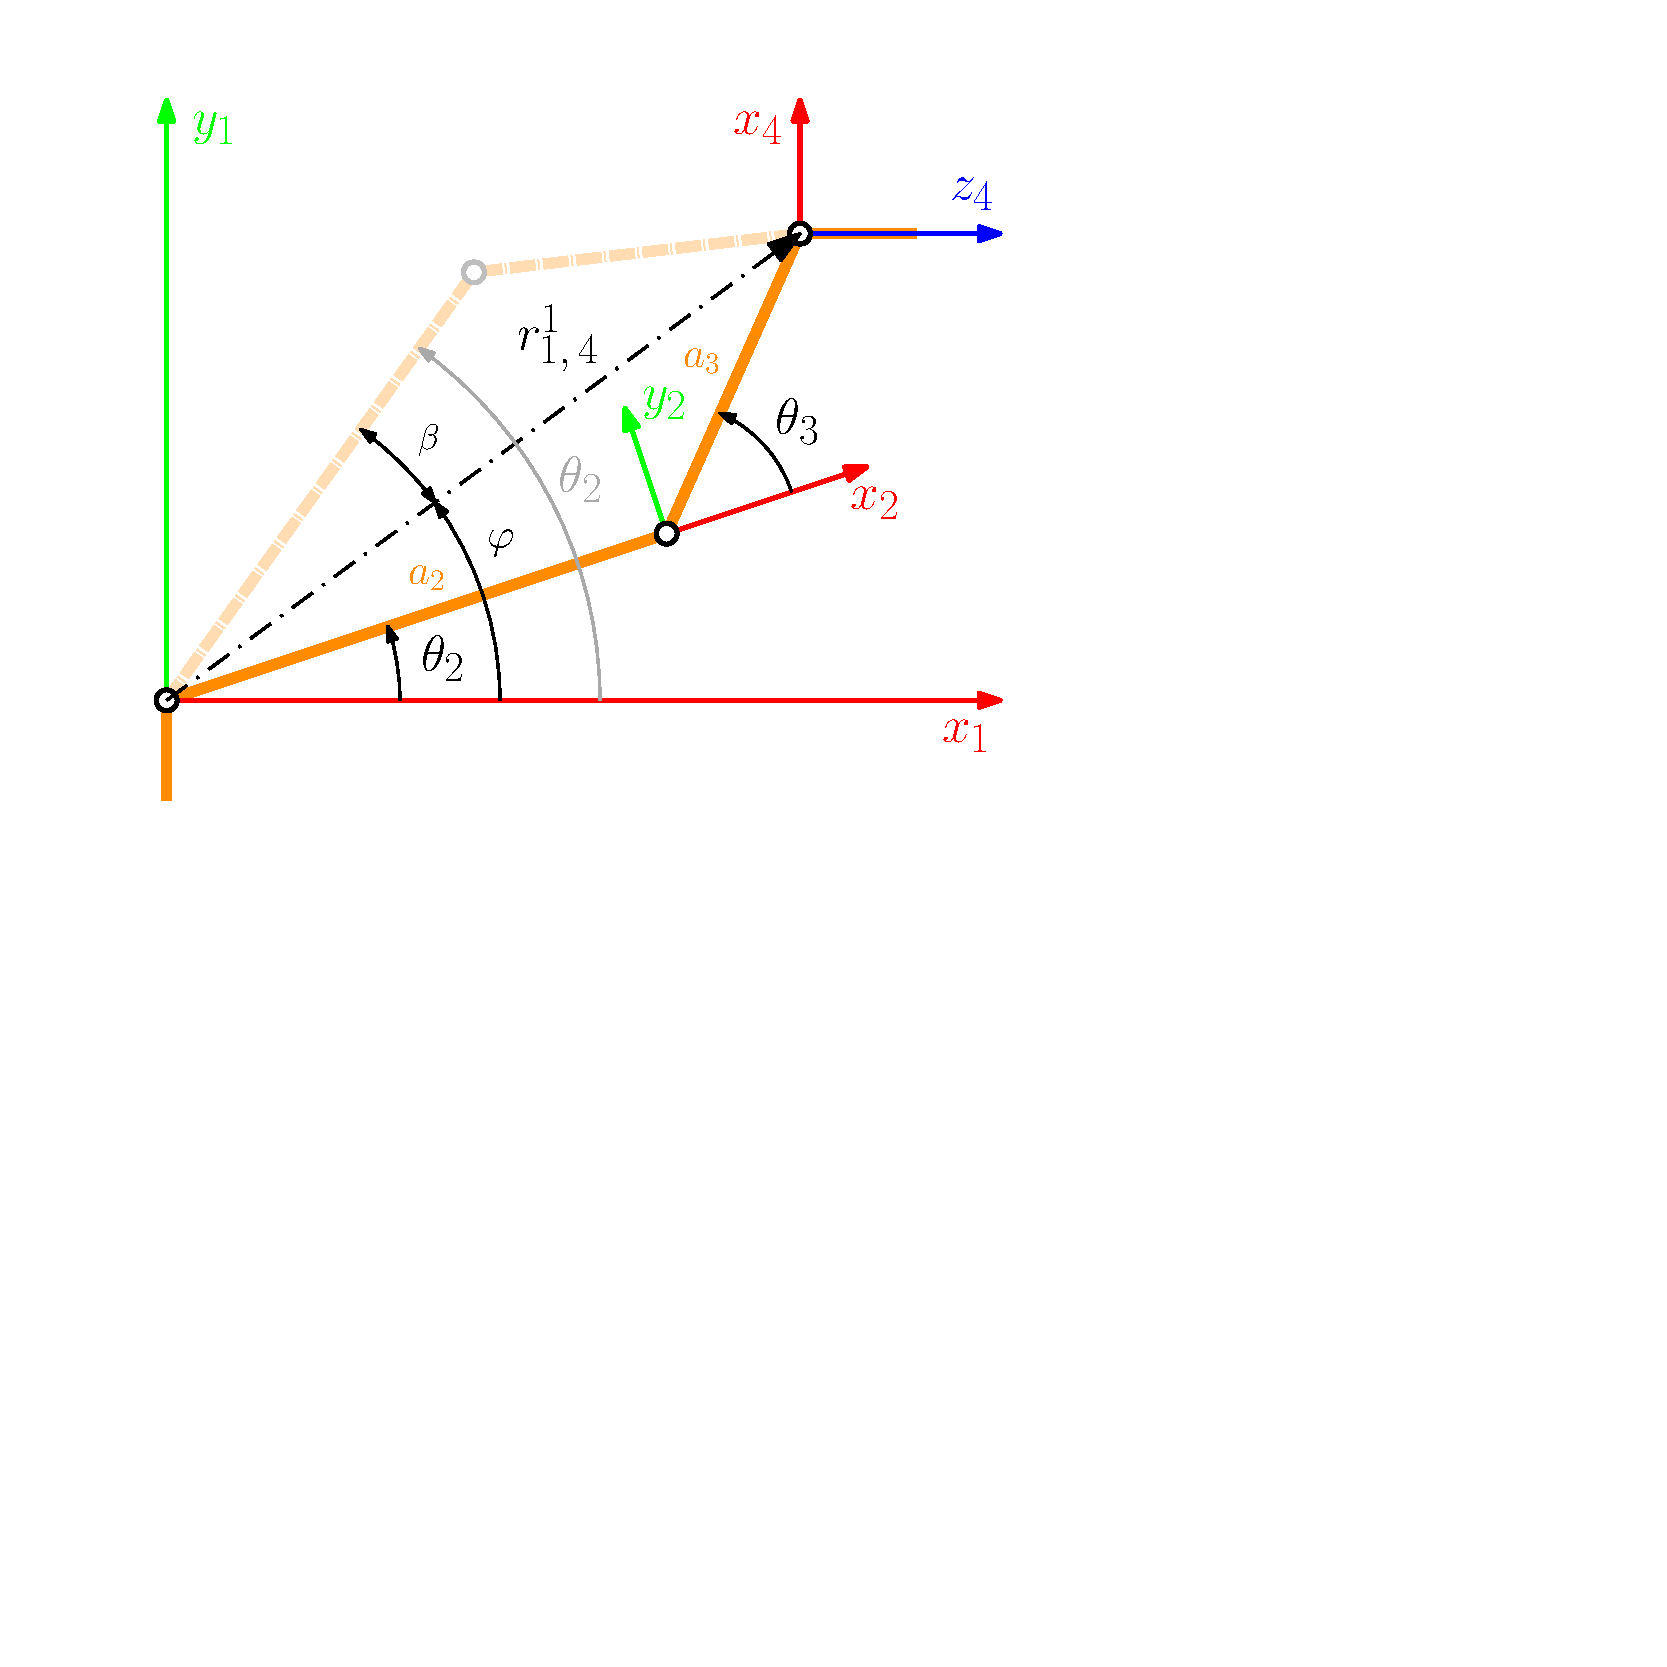
\includegraphics[width=0.7\textwidth]{ik_geometric_approach.pdf}
	\caption{Плоская часть манипулятора}
	\label{ik_geometric}
\end{figure}

Выпишем, пользуясь теоремой косинусов, выражения для $\theta_3$:
\begin{equation}
	\cos{\theta_3} = \frac{(^2p_4^x)^2 + (^2p_4^y)^2 + (^2p_4^z)^2 - a_3^2 - a_3^2}{2 a_3 a_4}
\end{equation}

\begin{equation}
	\theta_3^{1,2} = \mp Atan2(\sqrt{1 - \cos^2{\theta_3}}, \cos{\theta_3})
\end{equation}

Из рисунка~\ref{ik_geometric} видно, что, при $\theta_3 < 0$, $\theta_2 = \phi + \beta$:
\begin{equation}
	\theta_2^1 = Atan2(\sqrt{(^2p_4^x)^2 + (^2p_4^y)^2}, ^2p_4^z) + Atan2(a_4 \sin{\theta_3^1}, a_3 + a_4 \cos{\theta_3^1})
\end{equation}

При $\theta_3 > 0$, $\theta_2 = \phi - \beta$:
\begin{equation}
	\theta_2^2 = Atan2(\sqrt{(^2p_4^x)^2 + (^2p_4^y)^2}, ^2p_4^z) - Atan2(a_4 \sin{\theta_3^2}, a_3 + a_4 \cos{\theta_3^2})
\end{equation}

И, наконец:
\begin{equation}
	\theta_4^{1,2} = \theta_{234} - \theta_{2}^{1,2} - \theta_{3}^{1,2}
\end{equation}



\newpage